% Options for packages loaded elsewhere
\PassOptionsToPackage{unicode}{hyperref}
\PassOptionsToPackage{hyphens}{url}
\PassOptionsToPackage{dvipsnames,svgnames,x11names}{xcolor}
%
\documentclass[
  a4paper,
  DIV=11,
  numbers=noendperiod]{scrartcl}

\usepackage{amsmath,amssymb}
\usepackage{iftex}
\ifPDFTeX
  \usepackage[T1]{fontenc}
  \usepackage[utf8]{inputenc}
  \usepackage{textcomp} % provide euro and other symbols
\else % if luatex or xetex
  \usepackage{unicode-math}
  \defaultfontfeatures{Scale=MatchLowercase}
  \defaultfontfeatures[\rmfamily]{Ligatures=TeX,Scale=1}
\fi
\usepackage{lmodern}
\ifPDFTeX\else  
    % xetex/luatex font selection
\fi
% Use upquote if available, for straight quotes in verbatim environments
\IfFileExists{upquote.sty}{\usepackage{upquote}}{}
\IfFileExists{microtype.sty}{% use microtype if available
  \usepackage[]{microtype}
  \UseMicrotypeSet[protrusion]{basicmath} % disable protrusion for tt fonts
}{}
\makeatletter
\@ifundefined{KOMAClassName}{% if non-KOMA class
  \IfFileExists{parskip.sty}{%
    \usepackage{parskip}
  }{% else
    \setlength{\parindent}{0pt}
    \setlength{\parskip}{6pt plus 2pt minus 1pt}}
}{% if KOMA class
  \KOMAoptions{parskip=half}}
\makeatother
\usepackage{xcolor}
\setlength{\emergencystretch}{3em} % prevent overfull lines
\setcounter{secnumdepth}{5}
% Make \paragraph and \subparagraph free-standing
\ifx\paragraph\undefined\else
  \let\oldparagraph\paragraph
  \renewcommand{\paragraph}[1]{\oldparagraph{#1}\mbox{}}
\fi
\ifx\subparagraph\undefined\else
  \let\oldsubparagraph\subparagraph
  \renewcommand{\subparagraph}[1]{\oldsubparagraph{#1}\mbox{}}
\fi


\providecommand{\tightlist}{%
  \setlength{\itemsep}{0pt}\setlength{\parskip}{0pt}}\usepackage{longtable,booktabs,array}
\usepackage{calc} % for calculating minipage widths
% Correct order of tables after \paragraph or \subparagraph
\usepackage{etoolbox}
\makeatletter
\patchcmd\longtable{\par}{\if@noskipsec\mbox{}\fi\par}{}{}
\makeatother
% Allow footnotes in longtable head/foot
\IfFileExists{footnotehyper.sty}{\usepackage{footnotehyper}}{\usepackage{footnote}}
\makesavenoteenv{longtable}
\usepackage{graphicx}
\makeatletter
\def\maxwidth{\ifdim\Gin@nat@width>\linewidth\linewidth\else\Gin@nat@width\fi}
\def\maxheight{\ifdim\Gin@nat@height>\textheight\textheight\else\Gin@nat@height\fi}
\makeatother
% Scale images if necessary, so that they will not overflow the page
% margins by default, and it is still possible to overwrite the defaults
% using explicit options in \includegraphics[width, height, ...]{}
\setkeys{Gin}{width=\maxwidth,height=\maxheight,keepaspectratio}
% Set default figure placement to htbp
\makeatletter
\def\fps@figure{htbp}
\makeatother

\usepackage{fontspec}
\usepackage{multirow}
\usepackage{multicol}
\usepackage{colortbl}
\usepackage{hhline}
\newlength\Oldarrayrulewidth
\newlength\Oldtabcolsep
\usepackage{longtable}
\usepackage{array}
\usepackage{hyperref}
\usepackage{float}
\usepackage{wrapfig}
\usepackage{typearea}
\KOMAoption{captions}{tableheading}
\makeatletter
\makeatother
\makeatletter
\makeatother
\makeatletter
\@ifpackageloaded{caption}{}{\usepackage{caption}}
\AtBeginDocument{%
\ifdefined\contentsname
  \renewcommand*\contentsname{Índice}
\else
  \newcommand\contentsname{Índice}
\fi
\ifdefined\listfigurename
  \renewcommand*\listfigurename{Lista de Figuras}
\else
  \newcommand\listfigurename{Lista de Figuras}
\fi
\ifdefined\listtablename
  \renewcommand*\listtablename{Lista de Tabelas}
\else
  \newcommand\listtablename{Lista de Tabelas}
\fi
\ifdefined\figurename
  \renewcommand*\figurename{Figura}
\else
  \newcommand\figurename{Figura}
\fi
\ifdefined\tablename
  \renewcommand*\tablename{Tabela}
\else
  \newcommand\tablename{Tabela}
\fi
}
\@ifpackageloaded{float}{}{\usepackage{float}}
\floatstyle{ruled}
\@ifundefined{c@chapter}{\newfloat{codelisting}{h}{lop}}{\newfloat{codelisting}{h}{lop}[chapter]}
\floatname{codelisting}{Listagem}
\newcommand*\listoflistings{\listof{codelisting}{Lista de Listagens}}
\makeatother
\makeatletter
\@ifpackageloaded{caption}{}{\usepackage{caption}}
\@ifpackageloaded{subcaption}{}{\usepackage{subcaption}}
\makeatother
\makeatletter
\@ifpackageloaded{tcolorbox}{}{\usepackage[skins,breakable]{tcolorbox}}
\makeatother
\makeatletter
\@ifundefined{shadecolor}{\definecolor{shadecolor}{rgb}{.97, .97, .97}}
\makeatother
\makeatletter
\makeatother
\makeatletter
\makeatother
\ifLuaTeX
\usepackage[bidi=basic]{babel}
\else
\usepackage[bidi=default]{babel}
\fi
\babelprovide[main,import]{brazilian}
% get rid of language-specific shorthands (see #6817):
\let\LanguageShortHands\languageshorthands
\def\languageshorthands#1{}
\ifLuaTeX
  \usepackage{selnolig}  % disable illegal ligatures
\fi
\IfFileExists{bookmark.sty}{\usepackage{bookmark}}{\usepackage{hyperref}}
\IfFileExists{xurl.sty}{\usepackage{xurl}}{} % add URL line breaks if available
\urlstyle{same} % disable monospaced font for URLs
\hypersetup{
  pdflang={pt-br},
  colorlinks=true,
  linkcolor={blue},
  filecolor={Maroon},
  citecolor={Blue},
  urlcolor={Blue},
  pdfcreator={LaTeX via pandoc}}

\author{}
\date{}

\begin{document}
\ifdefined\Shaded\renewenvironment{Shaded}{\begin{tcolorbox}[breakable, frame hidden, sharp corners, boxrule=0pt, borderline west={3pt}{0pt}{shadecolor}, enhanced, interior hidden]}{\end{tcolorbox}}\fi

\thispagestyle{empty}
\begin{center}

\includegraphics[width=7cm]{logo_assec.png}
\end{center}
\vspace{3cm}
\begin{center}
\Huge\textbf{Avaliação dos Indicadores do PLS - Resolução CNJ Nº 400/2021} 
\end{center}
\begin{center}
\Huge\textbf{Consolidação dos dados mensais de 2023}
\end{center}
\begin{center}
\vspace{6cm}

\includegraphics[width=7cm]{logo_tre.png}
\end{center}
\begin{center}
\Large\textbf{2023}
\end{center}
\newpage
\tableofcontents
\newpage

\hypertarget{objetivo}{%
\section{Objetivo}\label{objetivo}}

Apresentar os resultados comparativos dos indicadores mensais
disponíveis do Plano de Logística Sustentável (Resolução CNJ Nº
400/2021) do ano de \textbf{2023}. Para efeito de comparação, serão
considerados dados referentes a 2021, ano em que havia ainda a
emergência sanitária global da Covid-19.

Serão indicados os resultados consolidados e representativos sobre o
consumo e/ou gastos com:

\begin{itemize}
\tightlist
\item
  Papel;
\item
  copos descartáveis;
\item
  água envasada em embalagens plásticas;
\item
  Impressão;
\item
  energia elétrica;
\item
  telefonia e;
\item
  gastos com serviços gráficos.
\end{itemize}

\hypertarget{papel-item-2}{%
\section{Papel (Item 2)}\label{papel-item-2}}

Os resultados relativos ao \textbf{item 2 - Papel} serão apresentados
considerando-se os indicadores \emph{2.1 - Consumo de papel próprio
(CPP)}, \emph{2.2 - Gasto com papel próprio (GPP)} e \emph{2.3 Consumo
de papel contratado (CPC)}.

\hypertarget{consumo-de-papel-pruxf3prio-2.1---cpp}{%
\subsection{Consumo de papel próprio (2.1 -
CPP)}\label{consumo-de-papel-pruxf3prio-2.1---cpp}}

\textbf{Definição}: quantidade de resmas de papel reciclado e não
reciclado, tamanhos A4 e Ofício, requisitada pelas unidades.

\textbf{Unidade de medida}: resmas.

A Tabela~\ref{tbl-tabcpp} apresenta a evolução mensal do indicador desde
2020.

\hypertarget{tbl-tabcpp}{}
\global\setlength{\Oldarrayrulewidth}{\arrayrulewidth}

\global\setlength{\Oldtabcolsep}{\tabcolsep}

\setlength{\tabcolsep}{0pt}

\renewcommand*{\arraystretch}{1.5}



\providecommand{\ascline}[3]{\noalign{\global\arrayrulewidth #1}\arrayrulecolor[HTML]{#2}\cline{#3}}

\begin{longtable}[c]{|p{0.58in}|p{0.60in}|p{0.67in}|p{0.60in}}
\caption{\label{tbl-tabcpp}Indicador 2.1 - Consumo de papel próprio (CPP) }\tabularnewline




\ascline{1,5pt}{666666}{1-4}

\multicolumn{1}{>{\centering}m{\dimexpr 0.58in+0\tabcolsep}}{\textcolor[HTML]{000000}{\fontsize{9}{9}\selectfont{\textbf{Mês}}}} & \multicolumn{1}{>{\centering}m{\dimexpr 0.6in+0\tabcolsep}}{\textcolor[HTML]{000000}{\fontsize{9}{9}\selectfont{\textbf{2021}}}} & \multicolumn{1}{>{\centering}m{\dimexpr 0.67in+0\tabcolsep}}{\textcolor[HTML]{000000}{\fontsize{9}{9}\selectfont{\textbf{2022}}}} & \multicolumn{1}{>{\centering}m{\dimexpr 0.6in+0\tabcolsep}}{\textcolor[HTML]{000000}{\fontsize{9}{9}\selectfont{\textbf{2023}}}} \\

\ascline{1,5pt}{666666}{1-4}\endfirsthead 

\ascline{1,5pt}{666666}{1-4}

\multicolumn{1}{>{\centering}m{\dimexpr 0.58in+0\tabcolsep}}{\textcolor[HTML]{000000}{\fontsize{9}{9}\selectfont{\textbf{Mês}}}} & \multicolumn{1}{>{\centering}m{\dimexpr 0.6in+0\tabcolsep}}{\textcolor[HTML]{000000}{\fontsize{9}{9}\selectfont{\textbf{2021}}}} & \multicolumn{1}{>{\centering}m{\dimexpr 0.67in+0\tabcolsep}}{\textcolor[HTML]{000000}{\fontsize{9}{9}\selectfont{\textbf{2022}}}} & \multicolumn{1}{>{\centering}m{\dimexpr 0.6in+0\tabcolsep}}{\textcolor[HTML]{000000}{\fontsize{9}{9}\selectfont{\textbf{2023}}}} \\

\ascline{1,5pt}{666666}{1-4}\endhead



\multicolumn{1}{>{\centering}m{\dimexpr 0.58in+0\tabcolsep}}{\textcolor[HTML]{000000}{\fontsize{9}{9}\selectfont{Jan}}} & \multicolumn{1}{>{\centering}m{\dimexpr 0.6in+0\tabcolsep}}{\textcolor[HTML]{000000}{\fontsize{9}{9}\selectfont{54}}} & \multicolumn{1}{>{\centering}m{\dimexpr 0.67in+0\tabcolsep}}{\textcolor[HTML]{000000}{\fontsize{9}{9}\selectfont{0}}} & \multicolumn{1}{>{\centering}m{\dimexpr 0.6in+0\tabcolsep}}{\textcolor[HTML]{000000}{\fontsize{9}{9}\selectfont{380}}} \\





\multicolumn{1}{>{\centering}m{\dimexpr 0.58in+0\tabcolsep}}{\textcolor[HTML]{000000}{\fontsize{9}{9}\selectfont{Fev}}} & \multicolumn{1}{>{\centering}m{\dimexpr 0.6in+0\tabcolsep}}{\textcolor[HTML]{000000}{\fontsize{9}{9}\selectfont{1.469}}} & \multicolumn{1}{>{\centering}m{\dimexpr 0.67in+0\tabcolsep}}{\textcolor[HTML]{000000}{\fontsize{9}{9}\selectfont{218}}} & \multicolumn{1}{>{\centering}m{\dimexpr 0.6in+0\tabcolsep}}{\textcolor[HTML]{000000}{\fontsize{9}{9}\selectfont{445}}} \\





\multicolumn{1}{>{\centering}m{\dimexpr 0.58in+0\tabcolsep}}{\textcolor[HTML]{000000}{\fontsize{9}{9}\selectfont{Mar}}} & \multicolumn{1}{>{\centering}m{\dimexpr 0.6in+0\tabcolsep}}{\textcolor[HTML]{000000}{\fontsize{9}{9}\selectfont{0}}} & \multicolumn{1}{>{\centering}m{\dimexpr 0.67in+0\tabcolsep}}{\textcolor[HTML]{000000}{\fontsize{9}{9}\selectfont{3.348}}} & \multicolumn{1}{>{\centering}m{\dimexpr 0.6in+0\tabcolsep}}{\textcolor[HTML]{000000}{\fontsize{9}{9}\selectfont{558}}} \\





\multicolumn{1}{>{\centering}m{\dimexpr 0.58in+0\tabcolsep}}{\textcolor[HTML]{000000}{\fontsize{9}{9}\selectfont{Abr}}} & \multicolumn{1}{>{\centering}m{\dimexpr 0.6in+0\tabcolsep}}{\textcolor[HTML]{000000}{\fontsize{9}{9}\selectfont{0}}} & \multicolumn{1}{>{\centering}m{\dimexpr 0.67in+0\tabcolsep}}{\textcolor[HTML]{000000}{\fontsize{9}{9}\selectfont{517}}} & \multicolumn{1}{>{\centering}m{\dimexpr 0.6in+0\tabcolsep}}{\textcolor[HTML]{000000}{\fontsize{9}{9}\selectfont{960}}} \\





\multicolumn{1}{>{\centering}m{\dimexpr 0.58in+0\tabcolsep}}{\textcolor[HTML]{000000}{\fontsize{9}{9}\selectfont{Mai}}} & \multicolumn{1}{>{\centering}m{\dimexpr 0.6in+0\tabcolsep}}{\textcolor[HTML]{000000}{\fontsize{9}{9}\selectfont{5}}} & \multicolumn{1}{>{\centering}m{\dimexpr 0.67in+0\tabcolsep}}{\textcolor[HTML]{000000}{\fontsize{9}{9}\selectfont{1.835}}} & \multicolumn{1}{>{\centering}m{\dimexpr 0.6in+0\tabcolsep}}{\textcolor[HTML]{000000}{\fontsize{9}{9}\selectfont{550}}} \\





\multicolumn{1}{>{\centering}m{\dimexpr 0.58in+0\tabcolsep}}{\textcolor[HTML]{000000}{\fontsize{9}{9}\selectfont{Jun}}} & \multicolumn{1}{>{\centering}m{\dimexpr 0.6in+0\tabcolsep}}{\textcolor[HTML]{000000}{\fontsize{9}{9}\selectfont{40}}} & \multicolumn{1}{>{\centering}m{\dimexpr 0.67in+0\tabcolsep}}{\textcolor[HTML]{000000}{\fontsize{9}{9}\selectfont{1.725}}} & \multicolumn{1}{>{\centering}m{\dimexpr 0.6in+0\tabcolsep}}{\textcolor[HTML]{000000}{\fontsize{9}{9}\selectfont{1.046}}} \\





\multicolumn{1}{>{\centering}m{\dimexpr 0.58in+0\tabcolsep}}{\textcolor[HTML]{000000}{\fontsize{9}{9}\selectfont{Jul}}} & \multicolumn{1}{>{\centering}m{\dimexpr 0.6in+0\tabcolsep}}{\textcolor[HTML]{000000}{\fontsize{9}{9}\selectfont{55}}} & \multicolumn{1}{>{\centering}m{\dimexpr 0.67in+0\tabcolsep}}{\textcolor[HTML]{000000}{\fontsize{9}{9}\selectfont{1.725}}} & \multicolumn{1}{>{\centering}m{\dimexpr 0.6in+0\tabcolsep}}{\textcolor[HTML]{000000}{\fontsize{9}{9}\selectfont{548}}} \\





\multicolumn{1}{>{\centering}m{\dimexpr 0.58in+0\tabcolsep}}{\textcolor[HTML]{000000}{\fontsize{9}{9}\selectfont{Ago}}} & \multicolumn{1}{>{\centering}m{\dimexpr 0.6in+0\tabcolsep}}{\textcolor[HTML]{000000}{\fontsize{9}{9}\selectfont{549}}} & \multicolumn{1}{>{\centering}m{\dimexpr 0.67in+0\tabcolsep}}{\textcolor[HTML]{000000}{\fontsize{9}{9}\selectfont{12.970}}} & \multicolumn{1}{>{\centering}m{\dimexpr 0.6in+0\tabcolsep}}{\textcolor[HTML]{000000}{\fontsize{9}{9}\selectfont{908}}} \\





\multicolumn{1}{>{\centering}m{\dimexpr 0.58in+0\tabcolsep}}{\textcolor[HTML]{000000}{\fontsize{9}{9}\selectfont{Set}}} & \multicolumn{1}{>{\centering}m{\dimexpr 0.6in+0\tabcolsep}}{\textcolor[HTML]{000000}{\fontsize{9}{9}\selectfont{1.082}}} & \multicolumn{1}{>{\centering}m{\dimexpr 0.67in+0\tabcolsep}}{\textcolor[HTML]{000000}{\fontsize{9}{9}\selectfont{4.773}}} & \multicolumn{1}{>{\centering}m{\dimexpr 0.6in+0\tabcolsep}}{\textcolor[HTML]{000000}{\fontsize{9}{9}\selectfont{1.155}}} \\





\multicolumn{1}{>{\centering}m{\dimexpr 0.58in+0\tabcolsep}}{\textcolor[HTML]{000000}{\fontsize{9}{9}\selectfont{Out}}} & \multicolumn{1}{>{\centering}m{\dimexpr 0.6in+0\tabcolsep}}{\textcolor[HTML]{000000}{\fontsize{9}{9}\selectfont{700}}} & \multicolumn{1}{>{\centering}m{\dimexpr 0.67in+0\tabcolsep}}{\textcolor[HTML]{000000}{\fontsize{9}{9}\selectfont{1.635}}} & \multicolumn{1}{>{\centering}m{\dimexpr 0.6in+0\tabcolsep}}{\textcolor[HTML]{000000}{\fontsize{9}{9}\selectfont{2.956}}} \\





\multicolumn{1}{>{\centering}m{\dimexpr 0.58in+0\tabcolsep}}{\textcolor[HTML]{000000}{\fontsize{9}{9}\selectfont{Nov}}} & \multicolumn{1}{>{\centering}m{\dimexpr 0.6in+0\tabcolsep}}{\textcolor[HTML]{000000}{\fontsize{9}{9}\selectfont{2.255}}} & \multicolumn{1}{>{\centering}m{\dimexpr 0.67in+0\tabcolsep}}{\textcolor[HTML]{000000}{\fontsize{9}{9}\selectfont{2.322}}} & \multicolumn{1}{>{\centering}m{\dimexpr 0.6in+0\tabcolsep}}{\textcolor[HTML]{000000}{\fontsize{9}{9}\selectfont{188}}} \\





\multicolumn{1}{>{\centering}m{\dimexpr 0.58in+0\tabcolsep}}{\textcolor[HTML]{000000}{\fontsize{9}{9}\selectfont{Dez}}} & \multicolumn{1}{>{\centering}m{\dimexpr 0.6in+0\tabcolsep}}{\textcolor[HTML]{000000}{\fontsize{9}{9}\selectfont{20}}} & \multicolumn{1}{>{\centering}m{\dimexpr 0.67in+0\tabcolsep}}{\textcolor[HTML]{000000}{\fontsize{9}{9}\selectfont{115}}} & \multicolumn{1}{>{\centering}m{\dimexpr 0.6in+0\tabcolsep}}{\textcolor[HTML]{000000}{\fontsize{9}{9}\selectfont{31}}} \\





\multicolumn{1}{>{\centering}m{\dimexpr 0.58in+0\tabcolsep}}{\textcolor[HTML]{000000}{\fontsize{9}{9}\selectfont{\textbf{Total}}}} & \multicolumn{1}{>{\centering}m{\dimexpr 0.6in+0\tabcolsep}}{\textcolor[HTML]{000000}{\fontsize{9}{9}\selectfont{\textbf{6.229}}}} & \multicolumn{1}{>{\centering}m{\dimexpr 0.67in+0\tabcolsep}}{\textcolor[HTML]{000000}{\fontsize{9}{9}\selectfont{\textbf{31.183}}}} & \multicolumn{1}{>{\centering}m{\dimexpr 0.6in+0\tabcolsep}}{\textcolor[HTML]{000000}{\fontsize{9}{9}\selectfont{\textbf{9.725}}}} \\

\ascline{1,5pt}{666666}{1-4}



\end{longtable}



\arrayrulecolor[HTML]{000000}

\global\setlength{\arrayrulewidth}{\Oldarrayrulewidth}

\global\setlength{\tabcolsep}{\Oldtabcolsep}

\renewcommand*{\arraystretch}{1}

A Figura~\ref{fig-gcpp} e Figura~\ref{fig-gcppac} representam o
desempenho do indicador nos anos em estudo e os acumulados anuais,
respectivamente.

\begin{figure}[H]

{\centering 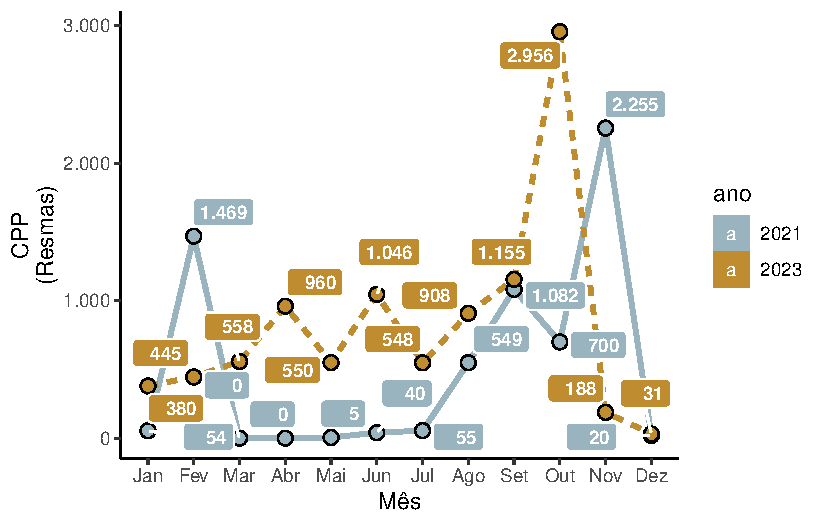
\includegraphics{relatorio_2023_files/figure-pdf/fig-gcpp-1.pdf}

}

\caption{\label{fig-gcpp}2.1 - CPP - 2021 e 2023}

\end{figure}

\begin{figure}[H]

{\centering 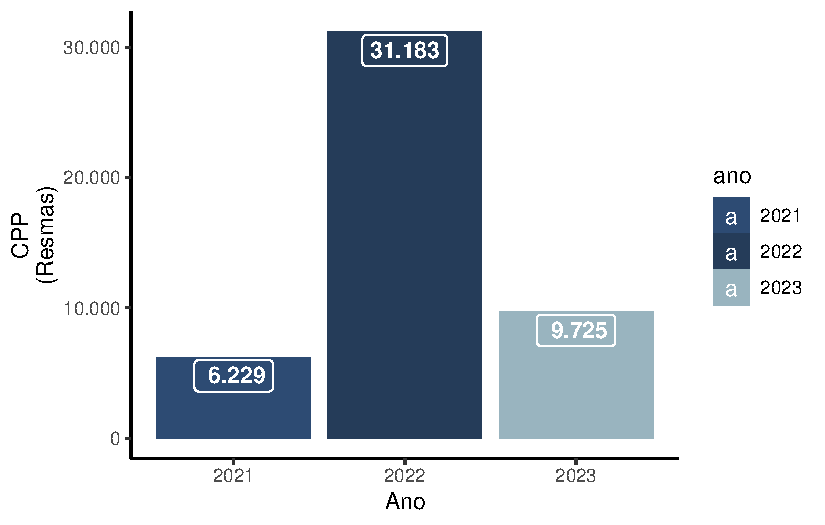
\includegraphics{relatorio_2023_files/figure-pdf/fig-gcppac-1.pdf}

}

\caption{\label{fig-gcppac}2.1 - CPP - acumulados anuais - 2021 a 2023}

\end{figure}

O agregado anual do consumo de papel total em 2023 foi de 9.725 resmas,
e no mesmo período de 2021, 6.229, o que acarreta no \textbf{aumento} de
\text{56,1}\% entre esses dois períodos analisados.

\hypertarget{gasto-com-papel-pruxf3prio-2.2---gpp}{%
\subsection{Gasto com Papel Próprio (2.2 -
GPP)}\label{gasto-com-papel-pruxf3prio-2.2---gpp}}

\textbf{Definição}: Despesa realizada com a aquisição de resmas de papel
reciclado e não reciclado, tamanhos A4 e Ofício. Considera-se evento
gerador a data da compra pelo órgão, conforme regime de competência.

\textbf{Unidade de medida}: reais.

A Tabela~\ref{tbl-tabgpp} apresenta a evolução mensal do indicador desde
2020.

\hypertarget{tbl-tabgpp}{}
\global\setlength{\Oldarrayrulewidth}{\arrayrulewidth}

\global\setlength{\Oldtabcolsep}{\tabcolsep}

\setlength{\tabcolsep}{0pt}

\renewcommand*{\arraystretch}{1.5}



\providecommand{\ascline}[3]{\noalign{\global\arrayrulewidth #1}\arrayrulecolor[HTML]{#2}\cline{#3}}

\begin{longtable}[c]{|p{0.58in}|p{0.84in}|p{0.74in}|p{0.84in}}
\caption{\label{tbl-tabgpp}Indicador 2.2 - Gasto com papel próprio (GPP) }\tabularnewline




\ascline{1,5pt}{666666}{1-4}

\multicolumn{1}{>{\centering}m{\dimexpr 0.58in+0\tabcolsep}}{\textcolor[HTML]{000000}{\fontsize{9}{9}\selectfont{\textbf{Mês}}}} & \multicolumn{1}{>{\centering}m{\dimexpr 0.84in+0\tabcolsep}}{\textcolor[HTML]{000000}{\fontsize{9}{9}\selectfont{\textbf{2021}}}} & \multicolumn{1}{>{\centering}m{\dimexpr 0.74in+0\tabcolsep}}{\textcolor[HTML]{000000}{\fontsize{9}{9}\selectfont{\textbf{2022}}}} & \multicolumn{1}{>{\centering}m{\dimexpr 0.84in+0\tabcolsep}}{\textcolor[HTML]{000000}{\fontsize{9}{9}\selectfont{\textbf{2023}}}} \\

\ascline{1,5pt}{666666}{1-4}\endfirsthead 

\ascline{1,5pt}{666666}{1-4}

\multicolumn{1}{>{\centering}m{\dimexpr 0.58in+0\tabcolsep}}{\textcolor[HTML]{000000}{\fontsize{9}{9}\selectfont{\textbf{Mês}}}} & \multicolumn{1}{>{\centering}m{\dimexpr 0.84in+0\tabcolsep}}{\textcolor[HTML]{000000}{\fontsize{9}{9}\selectfont{\textbf{2021}}}} & \multicolumn{1}{>{\centering}m{\dimexpr 0.74in+0\tabcolsep}}{\textcolor[HTML]{000000}{\fontsize{9}{9}\selectfont{\textbf{2022}}}} & \multicolumn{1}{>{\centering}m{\dimexpr 0.84in+0\tabcolsep}}{\textcolor[HTML]{000000}{\fontsize{9}{9}\selectfont{\textbf{2023}}}} \\

\ascline{1,5pt}{666666}{1-4}\endhead



\multicolumn{1}{>{\centering}m{\dimexpr 0.58in+0\tabcolsep}}{\textcolor[HTML]{000000}{\fontsize{9}{9}\selectfont{Jan}}} & \multicolumn{1}{>{\centering}m{\dimexpr 0.84in+0\tabcolsep}}{\textcolor[HTML]{000000}{\fontsize{9}{9}\selectfont{700,54}}} & \multicolumn{1}{>{\centering}m{\dimexpr 0.74in+0\tabcolsep}}{\textcolor[HTML]{000000}{\fontsize{9}{9}\selectfont{0}}} & \multicolumn{1}{>{\centering}m{\dimexpr 0.84in+0\tabcolsep}}{\textcolor[HTML]{000000}{\fontsize{9}{9}\selectfont{175.947,4}}} \\





\multicolumn{1}{>{\centering}m{\dimexpr 0.58in+0\tabcolsep}}{\textcolor[HTML]{000000}{\fontsize{9}{9}\selectfont{Fev}}} & \multicolumn{1}{>{\centering}m{\dimexpr 0.84in+0\tabcolsep}}{\textcolor[HTML]{000000}{\fontsize{9}{9}\selectfont{19.057,66}}} & \multicolumn{1}{>{\centering}m{\dimexpr 0.74in+0\tabcolsep}}{\textcolor[HTML]{000000}{\fontsize{9}{9}\selectfont{0}}} & \multicolumn{1}{>{\centering}m{\dimexpr 0.84in+0\tabcolsep}}{\textcolor[HTML]{000000}{\fontsize{9}{9}\selectfont{0,0}}} \\





\multicolumn{1}{>{\centering}m{\dimexpr 0.58in+0\tabcolsep}}{\textcolor[HTML]{000000}{\fontsize{9}{9}\selectfont{Mar}}} & \multicolumn{1}{>{\centering}m{\dimexpr 0.84in+0\tabcolsep}}{\textcolor[HTML]{000000}{\fontsize{9}{9}\selectfont{0,00}}} & \multicolumn{1}{>{\centering}m{\dimexpr 0.74in+0\tabcolsep}}{\textcolor[HTML]{000000}{\fontsize{9}{9}\selectfont{0}}} & \multicolumn{1}{>{\centering}m{\dimexpr 0.84in+0\tabcolsep}}{\textcolor[HTML]{000000}{\fontsize{9}{9}\selectfont{0,0}}} \\





\multicolumn{1}{>{\centering}m{\dimexpr 0.58in+0\tabcolsep}}{\textcolor[HTML]{000000}{\fontsize{9}{9}\selectfont{Abr}}} & \multicolumn{1}{>{\centering}m{\dimexpr 0.84in+0\tabcolsep}}{\textcolor[HTML]{000000}{\fontsize{9}{9}\selectfont{0,00}}} & \multicolumn{1}{>{\centering}m{\dimexpr 0.74in+0\tabcolsep}}{\textcolor[HTML]{000000}{\fontsize{9}{9}\selectfont{0}}} & \multicolumn{1}{>{\centering}m{\dimexpr 0.84in+0\tabcolsep}}{\textcolor[HTML]{000000}{\fontsize{9}{9}\selectfont{0,0}}} \\





\multicolumn{1}{>{\centering}m{\dimexpr 0.58in+0\tabcolsep}}{\textcolor[HTML]{000000}{\fontsize{9}{9}\selectfont{Mai}}} & \multicolumn{1}{>{\centering}m{\dimexpr 0.84in+0\tabcolsep}}{\textcolor[HTML]{000000}{\fontsize{9}{9}\selectfont{64,91}}} & \multicolumn{1}{>{\centering}m{\dimexpr 0.74in+0\tabcolsep}}{\textcolor[HTML]{000000}{\fontsize{9}{9}\selectfont{0}}} & \multicolumn{1}{>{\centering}m{\dimexpr 0.84in+0\tabcolsep}}{\textcolor[HTML]{000000}{\fontsize{9}{9}\selectfont{0,0}}} \\





\multicolumn{1}{>{\centering}m{\dimexpr 0.58in+0\tabcolsep}}{\textcolor[HTML]{000000}{\fontsize{9}{9}\selectfont{Jun}}} & \multicolumn{1}{>{\centering}m{\dimexpr 0.84in+0\tabcolsep}}{\textcolor[HTML]{000000}{\fontsize{9}{9}\selectfont{519,28}}} & \multicolumn{1}{>{\centering}m{\dimexpr 0.74in+0\tabcolsep}}{\textcolor[HTML]{000000}{\fontsize{9}{9}\selectfont{0}}} & \multicolumn{1}{>{\centering}m{\dimexpr 0.84in+0\tabcolsep}}{\textcolor[HTML]{000000}{\fontsize{9}{9}\selectfont{0,0}}} \\





\multicolumn{1}{>{\centering}m{\dimexpr 0.58in+0\tabcolsep}}{\textcolor[HTML]{000000}{\fontsize{9}{9}\selectfont{Jul}}} & \multicolumn{1}{>{\centering}m{\dimexpr 0.84in+0\tabcolsep}}{\textcolor[HTML]{000000}{\fontsize{9}{9}\selectfont{714,01}}} & \multicolumn{1}{>{\centering}m{\dimexpr 0.74in+0\tabcolsep}}{\textcolor[HTML]{000000}{\fontsize{9}{9}\selectfont{0}}} & \multicolumn{1}{>{\centering}m{\dimexpr 0.84in+0\tabcolsep}}{\textcolor[HTML]{000000}{\fontsize{9}{9}\selectfont{0,0}}} \\





\multicolumn{1}{>{\centering}m{\dimexpr 0.58in+0\tabcolsep}}{\textcolor[HTML]{000000}{\fontsize{9}{9}\selectfont{Ago}}} & \multicolumn{1}{>{\centering}m{\dimexpr 0.84in+0\tabcolsep}}{\textcolor[HTML]{000000}{\fontsize{9}{9}\selectfont{7.127,06}}} & \multicolumn{1}{>{\centering}m{\dimexpr 0.74in+0\tabcolsep}}{\textcolor[HTML]{000000}{\fontsize{9}{9}\selectfont{0}}} & \multicolumn{1}{>{\centering}m{\dimexpr 0.84in+0\tabcolsep}}{\textcolor[HTML]{000000}{\fontsize{9}{9}\selectfont{0,0}}} \\





\multicolumn{1}{>{\centering}m{\dimexpr 0.58in+0\tabcolsep}}{\textcolor[HTML]{000000}{\fontsize{9}{9}\selectfont{Set}}} & \multicolumn{1}{>{\centering}m{\dimexpr 0.84in+0\tabcolsep}}{\textcolor[HTML]{000000}{\fontsize{9}{9}\selectfont{14.046,46}}} & \multicolumn{1}{>{\centering}m{\dimexpr 0.74in+0\tabcolsep}}{\textcolor[HTML]{000000}{\fontsize{9}{9}\selectfont{0}}} & \multicolumn{1}{>{\centering}m{\dimexpr 0.84in+0\tabcolsep}}{\textcolor[HTML]{000000}{\fontsize{9}{9}\selectfont{0,0}}} \\





\multicolumn{1}{>{\centering}m{\dimexpr 0.58in+0\tabcolsep}}{\textcolor[HTML]{000000}{\fontsize{9}{9}\selectfont{Out}}} & \multicolumn{1}{>{\centering}m{\dimexpr 0.84in+0\tabcolsep}}{\textcolor[HTML]{000000}{\fontsize{9}{9}\selectfont{9.087,29}}} & \multicolumn{1}{>{\centering}m{\dimexpr 0.74in+0\tabcolsep}}{\textcolor[HTML]{000000}{\fontsize{9}{9}\selectfont{176.300}}} & \multicolumn{1}{>{\centering}m{\dimexpr 0.84in+0\tabcolsep}}{\textcolor[HTML]{000000}{\fontsize{9}{9}\selectfont{0,0}}} \\





\multicolumn{1}{>{\centering}m{\dimexpr 0.58in+0\tabcolsep}}{\textcolor[HTML]{000000}{\fontsize{9}{9}\selectfont{Nov}}} & \multicolumn{1}{>{\centering}m{\dimexpr 0.84in+0\tabcolsep}}{\textcolor[HTML]{000000}{\fontsize{9}{9}\selectfont{29.274,25}}} & \multicolumn{1}{>{\centering}m{\dimexpr 0.74in+0\tabcolsep}}{\textcolor[HTML]{000000}{\fontsize{9}{9}\selectfont{0}}} & \multicolumn{1}{>{\centering}m{\dimexpr 0.84in+0\tabcolsep}}{\textcolor[HTML]{000000}{\fontsize{9}{9}\selectfont{0,0}}} \\





\multicolumn{1}{>{\centering}m{\dimexpr 0.58in+0\tabcolsep}}{\textcolor[HTML]{000000}{\fontsize{9}{9}\selectfont{Dez}}} & \multicolumn{1}{>{\centering}m{\dimexpr 0.84in+0\tabcolsep}}{\textcolor[HTML]{000000}{\fontsize{9}{9}\selectfont{259,64}}} & \multicolumn{1}{>{\centering}m{\dimexpr 0.74in+0\tabcolsep}}{\textcolor[HTML]{000000}{\fontsize{9}{9}\selectfont{0}}} & \multicolumn{1}{>{\centering}m{\dimexpr 0.84in+0\tabcolsep}}{\textcolor[HTML]{000000}{\fontsize{9}{9}\selectfont{0,0}}} \\





\multicolumn{1}{>{\centering}m{\dimexpr 0.58in+0\tabcolsep}}{\textcolor[HTML]{000000}{\fontsize{9}{9}\selectfont{\textbf{Total}}}} & \multicolumn{1}{>{\centering}m{\dimexpr 0.84in+0\tabcolsep}}{\textcolor[HTML]{000000}{\fontsize{9}{9}\selectfont{\textbf{80.851,10}}}} & \multicolumn{1}{>{\centering}m{\dimexpr 0.74in+0\tabcolsep}}{\textcolor[HTML]{000000}{\fontsize{9}{9}\selectfont{\textbf{176.300}}}} & \multicolumn{1}{>{\centering}m{\dimexpr 0.84in+0\tabcolsep}}{\textcolor[HTML]{000000}{\fontsize{9}{9}\selectfont{\textbf{175.947,4}}}} \\

\ascline{1,5pt}{666666}{1-4}



\end{longtable}



\arrayrulecolor[HTML]{000000}

\global\setlength{\arrayrulewidth}{\Oldarrayrulewidth}

\global\setlength{\tabcolsep}{\Oldtabcolsep}

\renewcommand*{\arraystretch}{1}

O gasto de papel próprio em 2023 foi de R\$ 175.947,40 e em 2021, R\$
80.851,10, o que resultou no \textbf{aumento} de \text{117,6}\%. Em 2023
o gasto com papel foi anotado somente em janeiro.

A Figura~\ref{fig-ggpp} e Figura~\ref{fig-ggppac} representam o
desempenho do indicador nos anos em estudo e os acumulados anuais,
respectivamente.

\begin{figure}[H]

{\centering 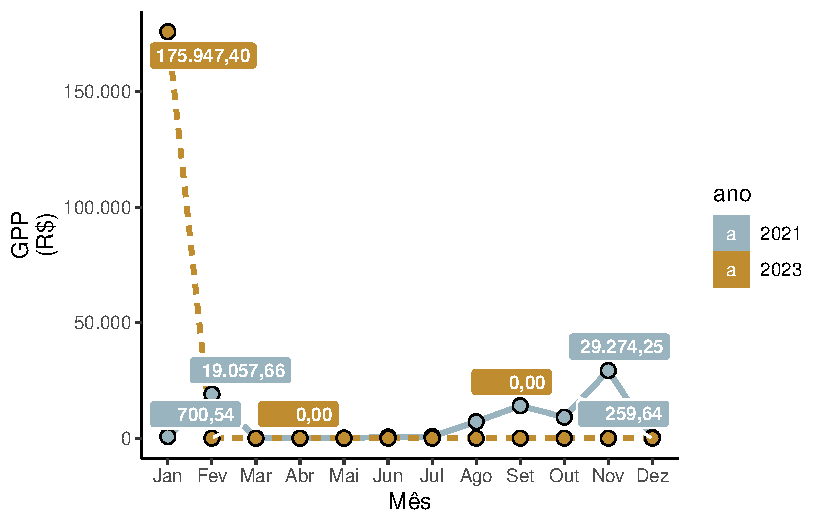
\includegraphics{relatorio_2023_files/figure-pdf/fig-ggpp-1.pdf}

}

\caption{\label{fig-ggpp}2.2 - GPP - 2021 e 2023}

\end{figure}

\begin{figure}[H]

{\centering 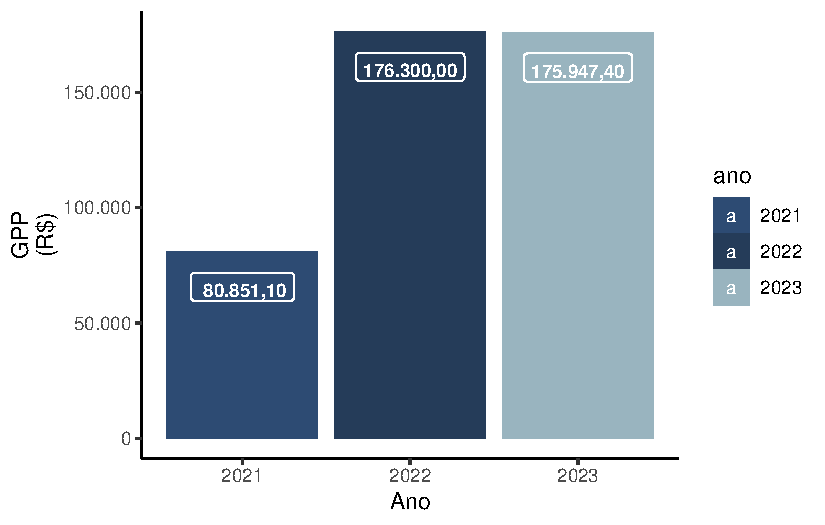
\includegraphics{relatorio_2023_files/figure-pdf/fig-ggppac-1.pdf}

}

\caption{\label{fig-ggppac}2.2 - GPP - acumulados anuais - 2021 a 2023}

\end{figure}

\hypertarget{consumo-de-papel-contratado-2.3---cpc}{%
\subsection{Consumo de Papel Contratado (2.3 -
CPC)}\label{consumo-de-papel-contratado-2.3---cpc}}

\textbf{Definição}: Quantidade total consumida de resmas de papel
reciclado e não reciclado, tamanhos A4 e Ofício, fornecidas por empresa
contratada para serviços de impressão e reprografia.

\textbf{Unidade de medida}: resmas.

\textbf{Não há informação de valores de consumo de papel contratado
entre 2021 a 2023.}

\newpage

\hypertarget{copos-descartuxe1veis-item-3}{%
\section{Copos Descartáveis (Item
3)}\label{copos-descartuxe1veis-item-3}}

Os resultados relativos ao \textbf{Item 3 - Copos Descartáveis} serão
apresentados considerando os indicadores \emph{3.1 - Consumo de copos
descartáveis (CC)} e \emph{3.2 - Gasto com copos descartáveis (GC)}.

\hypertarget{consumo-de-copos-descartuxe1veis-3.1---cc}{%
\subsection{Consumo de Copos Descartáveis (3.1 -
CC)}\label{consumo-de-copos-descartuxe1veis-3.1---cc}}

\textbf{Definição}: quantidade de copos descartáveis, usualmente
utilizados para consumo de água e café, requisitados pelas unidades.

\textbf{Unidade de medida}: centos.

A Tabela~\ref{tbl-tabcc} apresenta a evolução mensal do indicador desde
2021.

\hypertarget{tbl-tabcc}{}
\global\setlength{\Oldarrayrulewidth}{\arrayrulewidth}

\global\setlength{\Oldtabcolsep}{\tabcolsep}

\setlength{\tabcolsep}{0pt}

\renewcommand*{\arraystretch}{1.5}



\providecommand{\ascline}[3]{\noalign{\global\arrayrulewidth #1}\arrayrulecolor[HTML]{#2}\cline{#3}}

\begin{longtable}[c]{|p{0.58in}|p{0.60in}|p{0.60in}|p{0.56in}}
\caption{\label{tbl-tabcc}Indicador 3.1 - Consumo de copos descartáveis (CC) }\tabularnewline




\ascline{1,5pt}{666666}{1-4}

\multicolumn{1}{>{\centering}m{\dimexpr 0.58in+0\tabcolsep}}{\textcolor[HTML]{000000}{\fontsize{9}{9}\selectfont{\textbf{Mês}}}} & \multicolumn{1}{>{\centering}m{\dimexpr 0.6in+0\tabcolsep}}{\textcolor[HTML]{000000}{\fontsize{9}{9}\selectfont{\textbf{2021}}}} & \multicolumn{1}{>{\centering}m{\dimexpr 0.6in+0\tabcolsep}}{\textcolor[HTML]{000000}{\fontsize{9}{9}\selectfont{\textbf{2022}}}} & \multicolumn{1}{>{\centering}m{\dimexpr 0.56in+0\tabcolsep}}{\textcolor[HTML]{000000}{\fontsize{9}{9}\selectfont{\textbf{2023}}}} \\

\ascline{1,5pt}{666666}{1-4}\endfirsthead 

\ascline{1,5pt}{666666}{1-4}

\multicolumn{1}{>{\centering}m{\dimexpr 0.58in+0\tabcolsep}}{\textcolor[HTML]{000000}{\fontsize{9}{9}\selectfont{\textbf{Mês}}}} & \multicolumn{1}{>{\centering}m{\dimexpr 0.6in+0\tabcolsep}}{\textcolor[HTML]{000000}{\fontsize{9}{9}\selectfont{\textbf{2021}}}} & \multicolumn{1}{>{\centering}m{\dimexpr 0.6in+0\tabcolsep}}{\textcolor[HTML]{000000}{\fontsize{9}{9}\selectfont{\textbf{2022}}}} & \multicolumn{1}{>{\centering}m{\dimexpr 0.56in+0\tabcolsep}}{\textcolor[HTML]{000000}{\fontsize{9}{9}\selectfont{\textbf{2023}}}} \\

\ascline{1,5pt}{666666}{1-4}\endhead



\multicolumn{1}{>{\centering}m{\dimexpr 0.58in+0\tabcolsep}}{\textcolor[HTML]{000000}{\fontsize{9}{9}\selectfont{Jan}}} & \multicolumn{1}{>{\centering}m{\dimexpr 0.6in+0\tabcolsep}}{\textcolor[HTML]{000000}{\fontsize{9}{9}\selectfont{0}}} & \multicolumn{1}{>{\centering}m{\dimexpr 0.6in+0\tabcolsep}}{\textcolor[HTML]{000000}{\fontsize{9}{9}\selectfont{0}}} & \multicolumn{1}{>{\centering}m{\dimexpr 0.56in+0\tabcolsep}}{\textcolor[HTML]{000000}{\fontsize{9}{9}\selectfont{0}}} \\





\multicolumn{1}{>{\centering}m{\dimexpr 0.58in+0\tabcolsep}}{\textcolor[HTML]{000000}{\fontsize{9}{9}\selectfont{Fev}}} & \multicolumn{1}{>{\centering}m{\dimexpr 0.6in+0\tabcolsep}}{\textcolor[HTML]{000000}{\fontsize{9}{9}\selectfont{650}}} & \multicolumn{1}{>{\centering}m{\dimexpr 0.6in+0\tabcolsep}}{\textcolor[HTML]{000000}{\fontsize{9}{9}\selectfont{524}}} & \multicolumn{1}{>{\centering}m{\dimexpr 0.56in+0\tabcolsep}}{\textcolor[HTML]{000000}{\fontsize{9}{9}\selectfont{0}}} \\





\multicolumn{1}{>{\centering}m{\dimexpr 0.58in+0\tabcolsep}}{\textcolor[HTML]{000000}{\fontsize{9}{9}\selectfont{Mar}}} & \multicolumn{1}{>{\centering}m{\dimexpr 0.6in+0\tabcolsep}}{\textcolor[HTML]{000000}{\fontsize{9}{9}\selectfont{0}}} & \multicolumn{1}{>{\centering}m{\dimexpr 0.6in+0\tabcolsep}}{\textcolor[HTML]{000000}{\fontsize{9}{9}\selectfont{1.805}}} & \multicolumn{1}{>{\centering}m{\dimexpr 0.56in+0\tabcolsep}}{\textcolor[HTML]{000000}{\fontsize{9}{9}\selectfont{0}}} \\





\multicolumn{1}{>{\centering}m{\dimexpr 0.58in+0\tabcolsep}}{\textcolor[HTML]{000000}{\fontsize{9}{9}\selectfont{Abr}}} & \multicolumn{1}{>{\centering}m{\dimexpr 0.6in+0\tabcolsep}}{\textcolor[HTML]{000000}{\fontsize{9}{9}\selectfont{0}}} & \multicolumn{1}{>{\centering}m{\dimexpr 0.6in+0\tabcolsep}}{\textcolor[HTML]{000000}{\fontsize{9}{9}\selectfont{403}}} & \multicolumn{1}{>{\centering}m{\dimexpr 0.56in+0\tabcolsep}}{\textcolor[HTML]{000000}{\fontsize{9}{9}\selectfont{0}}} \\





\multicolumn{1}{>{\centering}m{\dimexpr 0.58in+0\tabcolsep}}{\textcolor[HTML]{000000}{\fontsize{9}{9}\selectfont{Mai}}} & \multicolumn{1}{>{\centering}m{\dimexpr 0.6in+0\tabcolsep}}{\textcolor[HTML]{000000}{\fontsize{9}{9}\selectfont{500}}} & \multicolumn{1}{>{\centering}m{\dimexpr 0.6in+0\tabcolsep}}{\textcolor[HTML]{000000}{\fontsize{9}{9}\selectfont{679}}} & \multicolumn{1}{>{\centering}m{\dimexpr 0.56in+0\tabcolsep}}{\textcolor[HTML]{000000}{\fontsize{9}{9}\selectfont{0}}} \\





\multicolumn{1}{>{\centering}m{\dimexpr 0.58in+0\tabcolsep}}{\textcolor[HTML]{000000}{\fontsize{9}{9}\selectfont{Jun}}} & \multicolumn{1}{>{\centering}m{\dimexpr 0.6in+0\tabcolsep}}{\textcolor[HTML]{000000}{\fontsize{9}{9}\selectfont{37}}} & \multicolumn{1}{>{\centering}m{\dimexpr 0.6in+0\tabcolsep}}{\textcolor[HTML]{000000}{\fontsize{9}{9}\selectfont{383}}} & \multicolumn{1}{>{\centering}m{\dimexpr 0.56in+0\tabcolsep}}{\textcolor[HTML]{000000}{\fontsize{9}{9}\selectfont{0}}} \\





\multicolumn{1}{>{\centering}m{\dimexpr 0.58in+0\tabcolsep}}{\textcolor[HTML]{000000}{\fontsize{9}{9}\selectfont{Jul}}} & \multicolumn{1}{>{\centering}m{\dimexpr 0.6in+0\tabcolsep}}{\textcolor[HTML]{000000}{\fontsize{9}{9}\selectfont{200}}} & \multicolumn{1}{>{\centering}m{\dimexpr 0.6in+0\tabcolsep}}{\textcolor[HTML]{000000}{\fontsize{9}{9}\selectfont{590}}} & \multicolumn{1}{>{\centering}m{\dimexpr 0.56in+0\tabcolsep}}{\textcolor[HTML]{000000}{\fontsize{9}{9}\selectfont{0}}} \\





\multicolumn{1}{>{\centering}m{\dimexpr 0.58in+0\tabcolsep}}{\textcolor[HTML]{000000}{\fontsize{9}{9}\selectfont{Ago}}} & \multicolumn{1}{>{\centering}m{\dimexpr 0.6in+0\tabcolsep}}{\textcolor[HTML]{000000}{\fontsize{9}{9}\selectfont{2.901}}} & \multicolumn{1}{>{\centering}m{\dimexpr 0.6in+0\tabcolsep}}{\textcolor[HTML]{000000}{\fontsize{9}{9}\selectfont{820}}} & \multicolumn{1}{>{\centering}m{\dimexpr 0.56in+0\tabcolsep}}{\textcolor[HTML]{000000}{\fontsize{9}{9}\selectfont{0}}} \\





\multicolumn{1}{>{\centering}m{\dimexpr 0.58in+0\tabcolsep}}{\textcolor[HTML]{000000}{\fontsize{9}{9}\selectfont{Set}}} & \multicolumn{1}{>{\centering}m{\dimexpr 0.6in+0\tabcolsep}}{\textcolor[HTML]{000000}{\fontsize{9}{9}\selectfont{251}}} & \multicolumn{1}{>{\centering}m{\dimexpr 0.6in+0\tabcolsep}}{\textcolor[HTML]{000000}{\fontsize{9}{9}\selectfont{1.122}}} & \multicolumn{1}{>{\centering}m{\dimexpr 0.56in+0\tabcolsep}}{\textcolor[HTML]{000000}{\fontsize{9}{9}\selectfont{0}}} \\





\multicolumn{1}{>{\centering}m{\dimexpr 0.58in+0\tabcolsep}}{\textcolor[HTML]{000000}{\fontsize{9}{9}\selectfont{Out}}} & \multicolumn{1}{>{\centering}m{\dimexpr 0.6in+0\tabcolsep}}{\textcolor[HTML]{000000}{\fontsize{9}{9}\selectfont{10}}} & \multicolumn{1}{>{\centering}m{\dimexpr 0.6in+0\tabcolsep}}{\textcolor[HTML]{000000}{\fontsize{9}{9}\selectfont{371}}} & \multicolumn{1}{>{\centering}m{\dimexpr 0.56in+0\tabcolsep}}{\textcolor[HTML]{000000}{\fontsize{9}{9}\selectfont{0}}} \\





\multicolumn{1}{>{\centering}m{\dimexpr 0.58in+0\tabcolsep}}{\textcolor[HTML]{000000}{\fontsize{9}{9}\selectfont{Nov}}} & \multicolumn{1}{>{\centering}m{\dimexpr 0.6in+0\tabcolsep}}{\textcolor[HTML]{000000}{\fontsize{9}{9}\selectfont{1.144}}} & \multicolumn{1}{>{\centering}m{\dimexpr 0.6in+0\tabcolsep}}{\textcolor[HTML]{000000}{\fontsize{9}{9}\selectfont{0}}} & \multicolumn{1}{>{\centering}m{\dimexpr 0.56in+0\tabcolsep}}{\textcolor[HTML]{000000}{\fontsize{9}{9}\selectfont{0}}} \\





\multicolumn{1}{>{\centering}m{\dimexpr 0.58in+0\tabcolsep}}{\textcolor[HTML]{000000}{\fontsize{9}{9}\selectfont{Dez}}} & \multicolumn{1}{>{\centering}m{\dimexpr 0.6in+0\tabcolsep}}{\textcolor[HTML]{000000}{\fontsize{9}{9}\selectfont{0}}} & \multicolumn{1}{>{\centering}m{\dimexpr 0.6in+0\tabcolsep}}{\textcolor[HTML]{000000}{\fontsize{9}{9}\selectfont{0}}} & \multicolumn{1}{>{\centering}m{\dimexpr 0.56in+0\tabcolsep}}{\textcolor[HTML]{000000}{\fontsize{9}{9}\selectfont{0}}} \\





\multicolumn{1}{>{\centering}m{\dimexpr 0.58in+0\tabcolsep}}{\textcolor[HTML]{000000}{\fontsize{9}{9}\selectfont{\textbf{Total}}}} & \multicolumn{1}{>{\centering}m{\dimexpr 0.6in+0\tabcolsep}}{\textcolor[HTML]{000000}{\fontsize{9}{9}\selectfont{\textbf{5.693}}}} & \multicolumn{1}{>{\centering}m{\dimexpr 0.6in+0\tabcolsep}}{\textcolor[HTML]{000000}{\fontsize{9}{9}\selectfont{\textbf{6.697}}}} & \multicolumn{1}{>{\centering}m{\dimexpr 0.56in+0\tabcolsep}}{\textcolor[HTML]{000000}{\fontsize{9}{9}\selectfont{\textbf{0}}}} \\

\ascline{1,5pt}{666666}{1-4}



\end{longtable}



\arrayrulecolor[HTML]{000000}

\global\setlength{\arrayrulewidth}{\Oldarrayrulewidth}

\global\setlength{\tabcolsep}{\Oldtabcolsep}

\renewcommand*{\arraystretch}{1}

A Figura~\ref{fig-gcc} representa o desempenho do indicador nos anos de
2021 e 2023 e a Figura~\ref{fig-gccac} , os acumulados anuais do
indicador.

\begin{figure}[H]

{\centering 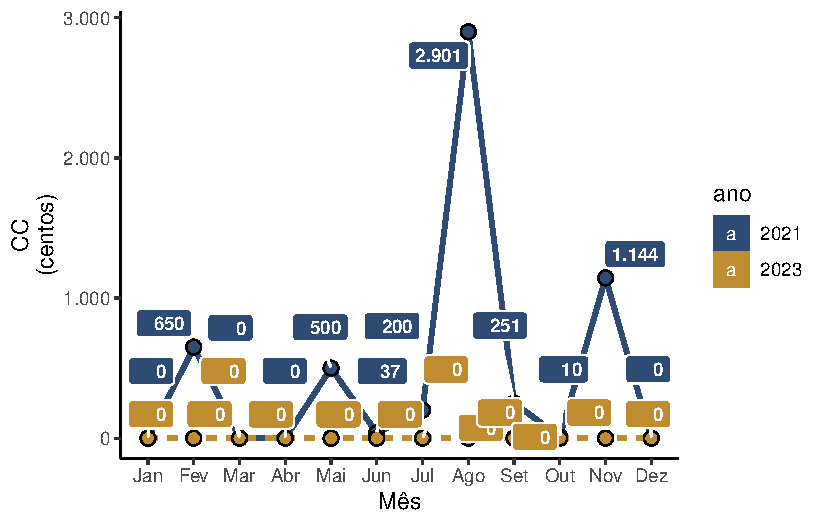
\includegraphics{relatorio_2023_files/figure-pdf/fig-gcc-1.pdf}

}

\caption{\label{fig-gcc}3.1 - CC - 2022}

\end{figure}

\begin{figure}[H]

{\centering 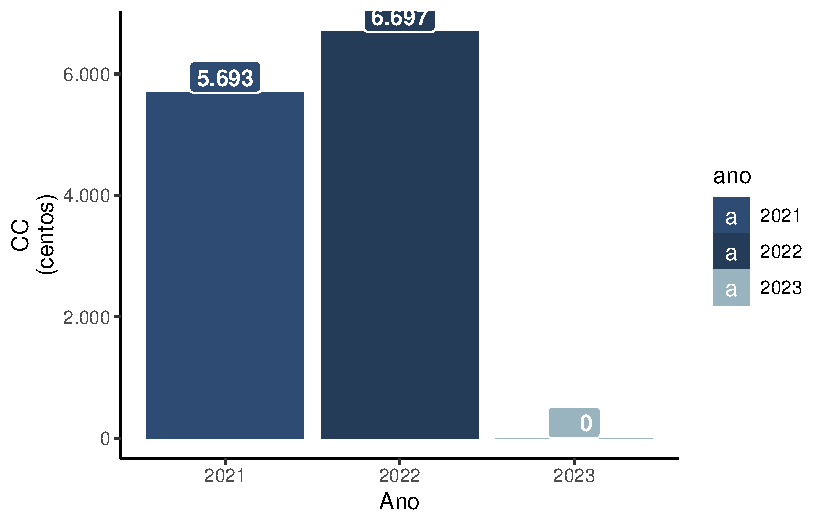
\includegraphics{relatorio_2023_files/figure-pdf/fig-gccac-1.pdf}

}

\caption{\label{fig-gccac}3.1 - CC - acumulados anuais - 2021 a 2023}

\end{figure}

\textbf{A partir de novembro de 2022, o TRE/SP passou a utilizar copos
biodegradáveis que não entram no cômputo do indicador.}

\hypertarget{gasto-de-copos-descartuxe1veis-3.2---gc}{%
\subsection{Gasto de Copos Descartáveis (3.2 -
GC)}\label{gasto-de-copos-descartuxe1veis-3.2---gc}}

\textbf{Definição}: despesa realizada com a aquisição de copos
descartáveis usualmente destinados para consumo de água e café.
Considera-se evento gerador a data da compra pelo órgão, conforme regime
de competência.

\textbf{Unidade de medida}: reais.

\textbf{Não há registros de gastos com copos descartáveis em 2021, 2022
e 2023.} A partir de novembro de 2022, o TRE/SP passou a utilizar copos
biodegradáveis que não entram no cômputo.

\newpage

\hypertarget{uxe1gua-envasada-em-embalagens-pluxe1sticas-item-4}{%
\section{Água Envasada em Embalagens Plásticas (Item
4)}\label{uxe1gua-envasada-em-embalagens-pluxe1sticas-item-4}}

As variáveis referentes ao \textbf{Item 4 - Água Envasada em Embalagens
Plásticas} serão apresentadas considerando-se os indicadores mensais
\emph{4.1 - Consumo de embalagens descartáveis para água mineral (CED)}
e \emph{4.2 - Consumo de embalagens retornáveis para água mineral
(CER)}, \emph{4.3 - Gasto com água mineral em embalagens descartáveis
(GAED)} e \emph{4.4 - Gasto com água mineral em embalagens retornáveis
(GAER)}.

\hypertarget{consumo-de-embalagens-descartuxe1veis-para-uxe1gua-mineral-4.1---ced}{%
\subsection{Consumo de embalagens descartáveis para água mineral (4.1 -
CED)}\label{consumo-de-embalagens-descartuxe1veis-para-uxe1gua-mineral-4.1---ced}}

\textbf{Definição}: quantidade de embalagens plásticas descartáveis de
água mineral (com ou sem gás) requisitada pelas unidades.

\textbf{Unidade de medida}: unidades.

A Tabela~\ref{tbl-tabced} apresenta a evolução mensal do indicador entre
2021 e 2023.

\hypertarget{tbl-tabced}{}
\global\setlength{\Oldarrayrulewidth}{\arrayrulewidth}

\global\setlength{\Oldtabcolsep}{\tabcolsep}

\setlength{\tabcolsep}{0pt}

\renewcommand*{\arraystretch}{1.5}



\providecommand{\ascline}[3]{\noalign{\global\arrayrulewidth #1}\arrayrulecolor[HTML]{#2}\cline{#3}}

\begin{longtable}[c]{|p{0.58in}|p{0.67in}|p{0.67in}|p{0.67in}}
\caption{\label{tbl-tabced}Indicador 4.1 - Consumo de embalagens descartáveis para água mineral
(CED) }\tabularnewline




\ascline{1,5pt}{666666}{1-4}

\multicolumn{1}{>{\centering}m{\dimexpr 0.58in+0\tabcolsep}}{\textcolor[HTML]{000000}{\fontsize{9}{9}\selectfont{\textbf{Mês}}}} & \multicolumn{1}{>{\centering}m{\dimexpr 0.67in+0\tabcolsep}}{\textcolor[HTML]{000000}{\fontsize{9}{9}\selectfont{\textbf{2021}}}} & \multicolumn{1}{>{\centering}m{\dimexpr 0.67in+0\tabcolsep}}{\textcolor[HTML]{000000}{\fontsize{9}{9}\selectfont{\textbf{2022}}}} & \multicolumn{1}{>{\centering}m{\dimexpr 0.67in+0\tabcolsep}}{\textcolor[HTML]{000000}{\fontsize{9}{9}\selectfont{\textbf{2023}}}} \\

\ascline{1,5pt}{666666}{1-4}\endfirsthead 

\ascline{1,5pt}{666666}{1-4}

\multicolumn{1}{>{\centering}m{\dimexpr 0.58in+0\tabcolsep}}{\textcolor[HTML]{000000}{\fontsize{9}{9}\selectfont{\textbf{Mês}}}} & \multicolumn{1}{>{\centering}m{\dimexpr 0.67in+0\tabcolsep}}{\textcolor[HTML]{000000}{\fontsize{9}{9}\selectfont{\textbf{2021}}}} & \multicolumn{1}{>{\centering}m{\dimexpr 0.67in+0\tabcolsep}}{\textcolor[HTML]{000000}{\fontsize{9}{9}\selectfont{\textbf{2022}}}} & \multicolumn{1}{>{\centering}m{\dimexpr 0.67in+0\tabcolsep}}{\textcolor[HTML]{000000}{\fontsize{9}{9}\selectfont{\textbf{2023}}}} \\

\ascline{1,5pt}{666666}{1-4}\endhead



\multicolumn{1}{>{\centering}m{\dimexpr 0.58in+0\tabcolsep}}{\textcolor[HTML]{000000}{\fontsize{9}{9}\selectfont{Jan}}} & \multicolumn{1}{>{\centering}m{\dimexpr 0.67in+0\tabcolsep}}{\textcolor[HTML]{000000}{\fontsize{9}{9}\selectfont{360}}} & \multicolumn{1}{>{\centering}m{\dimexpr 0.67in+0\tabcolsep}}{\textcolor[HTML]{000000}{\fontsize{9}{9}\selectfont{0}}} & \multicolumn{1}{>{\centering}m{\dimexpr 0.67in+0\tabcolsep}}{\textcolor[HTML]{000000}{\fontsize{9}{9}\selectfont{0}}} \\





\multicolumn{1}{>{\centering}m{\dimexpr 0.58in+0\tabcolsep}}{\textcolor[HTML]{000000}{\fontsize{9}{9}\selectfont{Fev}}} & \multicolumn{1}{>{\centering}m{\dimexpr 0.67in+0\tabcolsep}}{\textcolor[HTML]{000000}{\fontsize{9}{9}\selectfont{1.476}}} & \multicolumn{1}{>{\centering}m{\dimexpr 0.67in+0\tabcolsep}}{\textcolor[HTML]{000000}{\fontsize{9}{9}\selectfont{20}}} & \multicolumn{1}{>{\centering}m{\dimexpr 0.67in+0\tabcolsep}}{\textcolor[HTML]{000000}{\fontsize{9}{9}\selectfont{48}}} \\





\multicolumn{1}{>{\centering}m{\dimexpr 0.58in+0\tabcolsep}}{\textcolor[HTML]{000000}{\fontsize{9}{9}\selectfont{Mar}}} & \multicolumn{1}{>{\centering}m{\dimexpr 0.67in+0\tabcolsep}}{\textcolor[HTML]{000000}{\fontsize{9}{9}\selectfont{0}}} & \multicolumn{1}{>{\centering}m{\dimexpr 0.67in+0\tabcolsep}}{\textcolor[HTML]{000000}{\fontsize{9}{9}\selectfont{204}}} & \multicolumn{1}{>{\centering}m{\dimexpr 0.67in+0\tabcolsep}}{\textcolor[HTML]{000000}{\fontsize{9}{9}\selectfont{876}}} \\





\multicolumn{1}{>{\centering}m{\dimexpr 0.58in+0\tabcolsep}}{\textcolor[HTML]{000000}{\fontsize{9}{9}\selectfont{Abr}}} & \multicolumn{1}{>{\centering}m{\dimexpr 0.67in+0\tabcolsep}}{\textcolor[HTML]{000000}{\fontsize{9}{9}\selectfont{0}}} & \multicolumn{1}{>{\centering}m{\dimexpr 0.67in+0\tabcolsep}}{\textcolor[HTML]{000000}{\fontsize{9}{9}\selectfont{0}}} & \multicolumn{1}{>{\centering}m{\dimexpr 0.67in+0\tabcolsep}}{\textcolor[HTML]{000000}{\fontsize{9}{9}\selectfont{264}}} \\





\multicolumn{1}{>{\centering}m{\dimexpr 0.58in+0\tabcolsep}}{\textcolor[HTML]{000000}{\fontsize{9}{9}\selectfont{Mai}}} & \multicolumn{1}{>{\centering}m{\dimexpr 0.67in+0\tabcolsep}}{\textcolor[HTML]{000000}{\fontsize{9}{9}\selectfont{2.664}}} & \multicolumn{1}{>{\centering}m{\dimexpr 0.67in+0\tabcolsep}}{\textcolor[HTML]{000000}{\fontsize{9}{9}\selectfont{1.080}}} & \multicolumn{1}{>{\centering}m{\dimexpr 0.67in+0\tabcolsep}}{\textcolor[HTML]{000000}{\fontsize{9}{9}\selectfont{180}}} \\





\multicolumn{1}{>{\centering}m{\dimexpr 0.58in+0\tabcolsep}}{\textcolor[HTML]{000000}{\fontsize{9}{9}\selectfont{Jun}}} & \multicolumn{1}{>{\centering}m{\dimexpr 0.67in+0\tabcolsep}}{\textcolor[HTML]{000000}{\fontsize{9}{9}\selectfont{600}}} & \multicolumn{1}{>{\centering}m{\dimexpr 0.67in+0\tabcolsep}}{\textcolor[HTML]{000000}{\fontsize{9}{9}\selectfont{2.832}}} & \multicolumn{1}{>{\centering}m{\dimexpr 0.67in+0\tabcolsep}}{\textcolor[HTML]{000000}{\fontsize{9}{9}\selectfont{7.100}}} \\





\multicolumn{1}{>{\centering}m{\dimexpr 0.58in+0\tabcolsep}}{\textcolor[HTML]{000000}{\fontsize{9}{9}\selectfont{Jul}}} & \multicolumn{1}{>{\centering}m{\dimexpr 0.67in+0\tabcolsep}}{\textcolor[HTML]{000000}{\fontsize{9}{9}\selectfont{0}}} & \multicolumn{1}{>{\centering}m{\dimexpr 0.67in+0\tabcolsep}}{\textcolor[HTML]{000000}{\fontsize{9}{9}\selectfont{1.536}}} & \multicolumn{1}{>{\centering}m{\dimexpr 0.67in+0\tabcolsep}}{\textcolor[HTML]{000000}{\fontsize{9}{9}\selectfont{492}}} \\





\multicolumn{1}{>{\centering}m{\dimexpr 0.58in+0\tabcolsep}}{\textcolor[HTML]{000000}{\fontsize{9}{9}\selectfont{Ago}}} & \multicolumn{1}{>{\centering}m{\dimexpr 0.67in+0\tabcolsep}}{\textcolor[HTML]{000000}{\fontsize{9}{9}\selectfont{4.388}}} & \multicolumn{1}{>{\centering}m{\dimexpr 0.67in+0\tabcolsep}}{\textcolor[HTML]{000000}{\fontsize{9}{9}\selectfont{696}}} & \multicolumn{1}{>{\centering}m{\dimexpr 0.67in+0\tabcolsep}}{\textcolor[HTML]{000000}{\fontsize{9}{9}\selectfont{96}}} \\





\multicolumn{1}{>{\centering}m{\dimexpr 0.58in+0\tabcolsep}}{\textcolor[HTML]{000000}{\fontsize{9}{9}\selectfont{Set}}} & \multicolumn{1}{>{\centering}m{\dimexpr 0.67in+0\tabcolsep}}{\textcolor[HTML]{000000}{\fontsize{9}{9}\selectfont{414}}} & \multicolumn{1}{>{\centering}m{\dimexpr 0.67in+0\tabcolsep}}{\textcolor[HTML]{000000}{\fontsize{9}{9}\selectfont{2.712}}} & \multicolumn{1}{>{\centering}m{\dimexpr 0.67in+0\tabcolsep}}{\textcolor[HTML]{000000}{\fontsize{9}{9}\selectfont{564}}} \\





\multicolumn{1}{>{\centering}m{\dimexpr 0.58in+0\tabcolsep}}{\textcolor[HTML]{000000}{\fontsize{9}{9}\selectfont{Out}}} & \multicolumn{1}{>{\centering}m{\dimexpr 0.67in+0\tabcolsep}}{\textcolor[HTML]{000000}{\fontsize{9}{9}\selectfont{228}}} & \multicolumn{1}{>{\centering}m{\dimexpr 0.67in+0\tabcolsep}}{\textcolor[HTML]{000000}{\fontsize{9}{9}\selectfont{2.644}}} & \multicolumn{1}{>{\centering}m{\dimexpr 0.67in+0\tabcolsep}}{\textcolor[HTML]{000000}{\fontsize{9}{9}\selectfont{10.864}}} \\





\multicolumn{1}{>{\centering}m{\dimexpr 0.58in+0\tabcolsep}}{\textcolor[HTML]{000000}{\fontsize{9}{9}\selectfont{Nov}}} & \multicolumn{1}{>{\centering}m{\dimexpr 0.67in+0\tabcolsep}}{\textcolor[HTML]{000000}{\fontsize{9}{9}\selectfont{0}}} & \multicolumn{1}{>{\centering}m{\dimexpr 0.67in+0\tabcolsep}}{\textcolor[HTML]{000000}{\fontsize{9}{9}\selectfont{4.332}}} & \multicolumn{1}{>{\centering}m{\dimexpr 0.67in+0\tabcolsep}}{\textcolor[HTML]{000000}{\fontsize{9}{9}\selectfont{0}}} \\





\multicolumn{1}{>{\centering}m{\dimexpr 0.58in+0\tabcolsep}}{\textcolor[HTML]{000000}{\fontsize{9}{9}\selectfont{Dez}}} & \multicolumn{1}{>{\centering}m{\dimexpr 0.67in+0\tabcolsep}}{\textcolor[HTML]{000000}{\fontsize{9}{9}\selectfont{480}}} & \multicolumn{1}{>{\centering}m{\dimexpr 0.67in+0\tabcolsep}}{\textcolor[HTML]{000000}{\fontsize{9}{9}\selectfont{0}}} & \multicolumn{1}{>{\centering}m{\dimexpr 0.67in+0\tabcolsep}}{\textcolor[HTML]{000000}{\fontsize{9}{9}\selectfont{262}}} \\





\multicolumn{1}{>{\centering}m{\dimexpr 0.58in+0\tabcolsep}}{\textcolor[HTML]{000000}{\fontsize{9}{9}\selectfont{\textbf{Total}}}} & \multicolumn{1}{>{\centering}m{\dimexpr 0.67in+0\tabcolsep}}{\textcolor[HTML]{000000}{\fontsize{9}{9}\selectfont{\textbf{10.610}}}} & \multicolumn{1}{>{\centering}m{\dimexpr 0.67in+0\tabcolsep}}{\textcolor[HTML]{000000}{\fontsize{9}{9}\selectfont{\textbf{16.056}}}} & \multicolumn{1}{>{\centering}m{\dimexpr 0.67in+0\tabcolsep}}{\textcolor[HTML]{000000}{\fontsize{9}{9}\selectfont{\textbf{20.746}}}} \\

\ascline{1,5pt}{666666}{1-4}



\end{longtable}



\arrayrulecolor[HTML]{000000}

\global\setlength{\arrayrulewidth}{\Oldarrayrulewidth}

\global\setlength{\tabcolsep}{\Oldtabcolsep}

\renewcommand*{\arraystretch}{1}

\begin{figure}[H]

{\centering 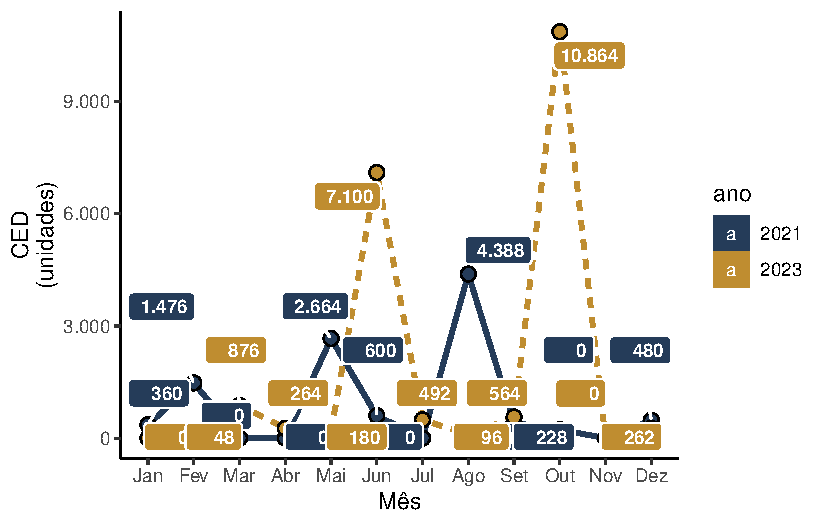
\includegraphics{relatorio_2023_files/figure-pdf/fig-gced-1.pdf}

}

\caption{\label{fig-gced}4.1 - CED - 2021 e 2023}

\end{figure}

A Figura~\ref{fig-gced} representa o desempenho do indicador em 2021 e
2023, e a Figura~\ref{fig-gcedac} , os acumulados anuais do indicador.

\begin{figure}[H]

{\centering 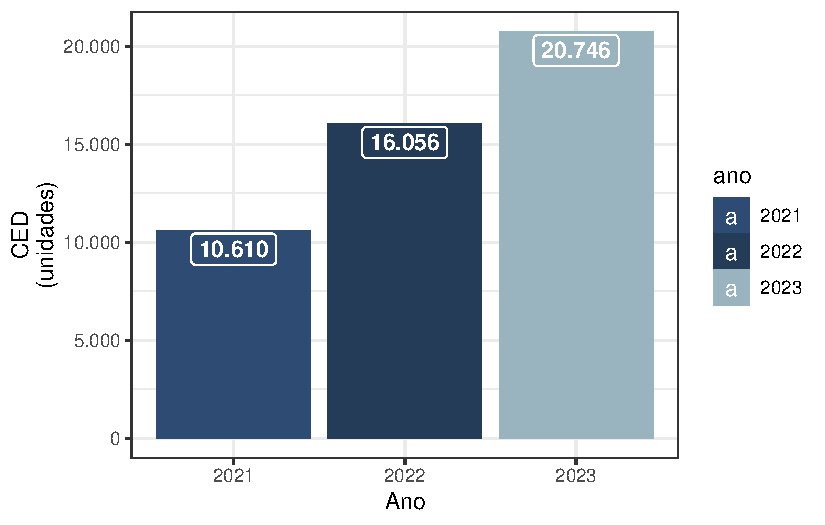
\includegraphics{relatorio_2023_files/figure-pdf/fig-gcedac-1.pdf}

}

\caption{\label{fig-gcedac}4.1- CED - acumulados anuais - 2021 a 2023}

\end{figure}

O consumo anual de embalagens descartáveis para água mineral foi, em
2023, de 20.746 unidades enquanto no ano de 2021, foi de 10.610, o que
resulta no \textbf{incremento} de \text{95,5}\% entre esses dois
períodos analisados.



\end{document}
